\documentclass{article}[18pt]
\ProvidesPackage{format}
%Page setup
\usepackage[utf8]{inputenc}
\usepackage[margin=0.7in]{geometry}
\usepackage{parselines} 
\usepackage[english]{babel}
\usepackage{fancyhdr}
\usepackage{titlesec}
\hyphenpenalty=10000

\pagestyle{fancy}
\fancyhf{}
\rhead{Sam Robbins}
\rfoot{Page \thepage}

%Characters
\usepackage{amsmath}
\usepackage{amssymb}
\usepackage{gensymb}
\newcommand{\R}{\mathbb{R}}

%Diagrams
\usepackage{pgfplots}
\usepackage{graphicx}
\usepackage{tabularx}
\usepackage{relsize}
\pgfplotsset{width=10cm,compat=1.9}
\usepackage{float}

%Length Setting
\titlespacing\section{0pt}{14pt plus 4pt minus 2pt}{0pt plus 2pt minus 2pt}
\newlength\tindent
\setlength{\tindent}{\parindent}
\setlength{\parindent}{0pt}
\renewcommand{\indent}{\hspace*{\tindent}}

%Programming Font
\usepackage{courier}
\usepackage{listings}
\usepackage{pxfonts}

%Lists
\usepackage{enumerate}
\usepackage{enumitem}

% Networks Macro
\usepackage{tikz}


% Commands for files converted using pandoc
\providecommand{\tightlist}{%
	\setlength{\itemsep}{0pt}\setlength{\parskip}{0pt}}
\usepackage{hyperref}

% Get nice commands for floor and ceil
\usepackage{mathtools}
\DeclarePairedDelimiter{\ceil}{\lceil}{\rceil}
\DeclarePairedDelimiter{\floor}{\lfloor}{\rfloor}

% Allow itemize to go up to 20 levels deep (just change the number if you need more you madman)
\usepackage{enumitem}
\setlistdepth{20}
\renewlist{itemize}{itemize}{20}

% initially, use dots for all levels
\setlist[itemize]{label=$\cdot$}

% customize the first 3 levels
\setlist[itemize,1]{label=\textbullet}
\setlist[itemize,2]{label=--}
\setlist[itemize,3]{label=*}

% Definition and Important Stuff
% Important stuff
\usepackage[framemethod=TikZ]{mdframed}

\newcounter{theo}[section]\setcounter{theo}{0}
\renewcommand{\thetheo}{\arabic{section}.\arabic{theo}}
\newenvironment{important}[1][]{%
	\refstepcounter{theo}%
	\ifstrempty{#1}%
	{\mdfsetup{%
			frametitle={%
				\tikz[baseline=(current bounding box.east),outer sep=0pt]
				\node[anchor=east,rectangle,fill=red!50]
				{\strut Important};}}
	}%
	{\mdfsetup{%
			frametitle={%
				\tikz[baseline=(current bounding box.east),outer sep=0pt]
				\node[anchor=east,rectangle,fill=red!50]
				{\strut Important:~#1};}}%
	}%
	\mdfsetup{innertopmargin=10pt,linecolor=red!50,%
		linewidth=2pt,topline=true,%
		frametitleaboveskip=\dimexpr-\ht\strutbox\relax
	}
	\begin{mdframed}[]\relax%
		\centering
		}{\end{mdframed}}



\newcounter{lem}[section]\setcounter{lem}{0}
\renewcommand{\thelem}{\arabic{section}.\arabic{lem}}
\newenvironment{defin}[1][]{%
	\refstepcounter{lem}%
	\ifstrempty{#1}%
	{\mdfsetup{%
			frametitle={%
				\tikz[baseline=(current bounding box.east),outer sep=0pt]
				\node[anchor=east,rectangle,fill=blue!20]
				{\strut Definition};}}
	}%
	{\mdfsetup{%
			frametitle={%
				\tikz[baseline=(current bounding box.east),outer sep=0pt]
				\node[anchor=east,rectangle,fill=blue!20]
				{\strut Definition:~#1};}}%
	}%
	\mdfsetup{innertopmargin=10pt,linecolor=blue!20,%
		linewidth=2pt,topline=true,%
		frametitleaboveskip=\dimexpr-\ht\strutbox\relax
	}
	\begin{mdframed}[]\relax%
		\centering
		}{\end{mdframed}}
\lhead{Software Engineering - Software Design}


\begin{document}
\begin{center}
\underline{\huge Software Design Patterns}
\end{center}
\section{Elements of a Design Pattern}
\begin{itemize}
	\item \textbf{Pattern Name} - A handle which aims to encapsulate a design pattern, its solutions and any consequences arising from its use
	\item \textbf{Problem} - When the pattern can be applied, and may include any conditions which must be met before it makes sense to apply that pattern
	\item \textbf{Solution} - Provides an abstract description of the elements that make up the design as well as their relationships and responsibilities
	\item \textbf{Consequences} - The results and trade-offs from applying the pattern
\end{itemize}
\section{The design pattern space}
Broadly classify by purpose using three groups
\begin{itemize}
	\item Creational patterns are concerned with the process of object creation
	\item Structural patterns are concerned with the composition of classes or objects
	\item Behavioural patterns characterise the ways in which classes or objects interact and distribute responsibility
\end{itemize}
Can also classify by scope
\section{Some characteristics}
\begin{itemize}
	\item Patterns tend to emphasise aggregation and interfaces over inheritance
	\item They aim to identify the parts of a system that are likely to change and to encapsulate those
	\item Patterns often aim for loose coupling, making for greater flexibility1
\end{itemize}
\section{Caveat to using patterns}
\begin{itemize}
	\item They are only of use to experts
	\item Inappropriate use of patterns cause problems for system maintenance 
	\item There is not a wide approval of patterns, people like to do things differently
\end{itemize}
\section{Proxy}
A proxy provides a surrogate or placeholder for another object to control access to it. 
\begin{center}
	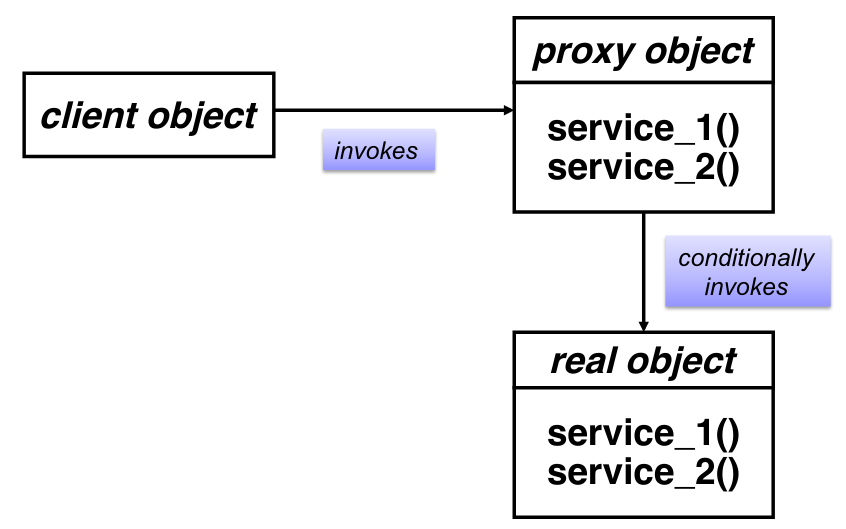
\includegraphics[scale=0.5]{Proxy}
\end{center}
A proxy is applicable wherever there is a need for a more versatile (and indirect) reference to an object than just a pointer. Examples of where this might be appropriate include:
\begin{itemize}
	\item \textbf{Remote proxy} - Provides a local representative for an object in a different address space
	\item \textbf{Virtual proxy} - creates "expensive" objects on demand, with an example being the "ImageProxy" described in the example of the word processor
	\item \textbf{Protection proxy} - Controls access to the original object, and is useful where users (objects) may have different access rights, depending on their role
	\item \textbf{Synchronisation Proxy} - Controls safe access to a subject from multiple threads
\end{itemize}
\section{Design Anti-Patterns}
\begin{itemize}
	\item Design anti-patterns describe obvious, but wrong solutions to recurring problems
	\item Focus tends to be a little different - anti-patterns are apt to be described in terms of the reasons why wrong solutions are adopted, rather than their form
\end{itemize}
\section{Code Smells}
\begin{itemize}
	\item These can be considered as a form of an anti-pattern
	\item A code smell is a design weakness that may form a future source of errors and that may contribute to the technical debt incurred when producing a design. Hence they act as a driver for refactoring
	\item Problem is to determine appropriate "boundaries"
\end{itemize}
\section{Documenting a design pattern}
Major headings:
\begin{itemize}
	\item Intent - what the pattern does
	\item Also Known As - Identifying any synonyms
	\item Motivation - why such a pattern is useful
	\item Applicability - Roles for the pattern
	\item Structure - Typically a class diagram
	\item Participants - Describing the classes in outline
	\item Collaborations - How the participants work together
	\item Consequences - benefits and liabilities of its use
	\item Implementation  - pitfalls, hints, language-specific issues
	\item Sample code - usually C++
	\item Known uses - Examples of successful application
	\item Related patterns - similar ones and how they differ
\end{itemize}
\section{Issues with design patterns}
\begin{itemize}
	\item [+] Attracted a strong body of support from a dedicated community of pattern enthusiasts
	\item [+] Provides a mechanism for reuse of design ideas, at least, for experts
	\item [+] Fairly standardised set of pattern names and description forms 
	\item [?] How many patterns can be realistically indexed and still be accessible to the designer
	\item [?] Is the idea one that is readily transferable to other architectural styles beyond O-O
	\item [?] Are they most likely to be effective when used for peer to peer exchange of knowledge
\end{itemize}
\section{Note}
Patterns need to be used with care:
\begin{itemize}
	\item Patterns may create an unnecessary overhead in terms of adding classes and code - so there has to be a justification for their use
	\item Code creating using patterns may be hard to understand
	\item Avoid using the singleton pattern (ensure a class has only one instance, and provide a global point of access to it) - can be mis-used to provide persistent data in a system
\end{itemize}
Hence patterns may be more use in identifying the form that a design solution might take, then in providing details of how it is to be implemented



\end{document}